
\FloatBarrier

\section{Система Дуффінга} % {{{1 _DUFF_
\label{atu:sect:duff}

\LinkRef{
 duff: ASAU-12, 15. APIR-2009. DSMP-2016
  % ~/doc/tex/asau/asau12/atu/atu.tex
  % ~/doc/tex/asau/asau15/atu/atu.tex
}

\subsection{Визначення системи та аналіз її динаміки} % {{{2

Розглянемо нелінійну динамічну систему Дуффінга~\cite{magni_theory_dyn_chaos,atu_asau12}:

\begin{equation}
 \ddot{x} + c_0 \dot{x} + \alpha x + \beta x^3 = u(t) ,
\label{atu:eq:duff}
\end{equation}
%
або її ж зі збереженням фізичних розмірностей:
%
\begin{equation}
 m \ddot{x} + \nu \dot{x} + k_1 x + k_3 x^3 = F(t) ,
\label{atu:eq:duff_phys}
\end{equation}

Тут
$ m $ --- маса об'єкта,
$ x (t) $ --- координата (вихідний сигнал),
$ u (t) = U_{in} \sin (\omega_{in} t) $ --- зовнішня сила,
$ k_1 $ --- коефіцієнт лінійної компоненти сили, що повертає,
$ k_3 $ --- коефіцієнт при нелінійної частини,
$ \alpha $ --- безрозмірний коефіцієнт лінійної компоненти сили, що повертає, при
$ \alpha> 0 $ і відсутності нелінійності визначає власну частоту: ($ \Omega_0^2 = \alpha $),
$ \nu $ і $ c_0 $ --- розмірний і безрозмірний коефіцієнти демпфірування,
$ \beta $ --- безрозмірний коефіцієнт нелінійної частини.

Ідентифікований параметр
$ \beta $ визначає нелінійні властивості системи. Слід зазначити,
що дана система проявляє хаотичні властивості тільки при малих
значеннях параметра \(c_0\). При більшому впливі дисипативної
складової система~(\ref{atu:eq:duff}) якісно не відрізняється від
лінійної коливальної системи, і для її ідентифікації застосовні
класичні критерії.


На рис.~\ref{atu:f:duff_phase_f_reg} наведено розширений фазовий портрет
і спектр системи Дуффінга в режимі складно-періодичних
коливань. Слід зазначити, що існують умови, при яких добавка до
гармонійного вхідного сигналу шумоподібної складової може
перевести систему в хаотичний режим~\cite{atu_asau15}.

\begin{figure}[ht!]
\begin{center}
  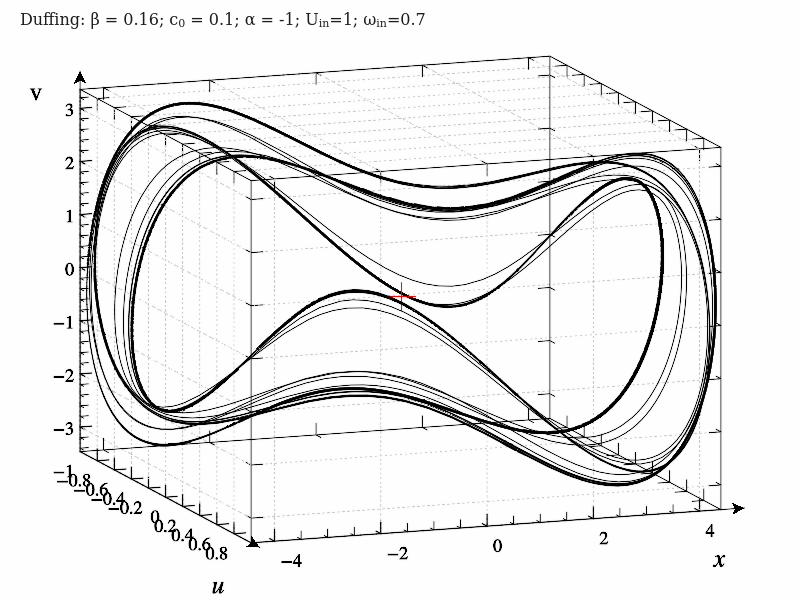
\includegraphics[width=0.49\textwidth]{p/cha/duff/duff_p_1x00_0x70_0x16.png}
  \hfill
  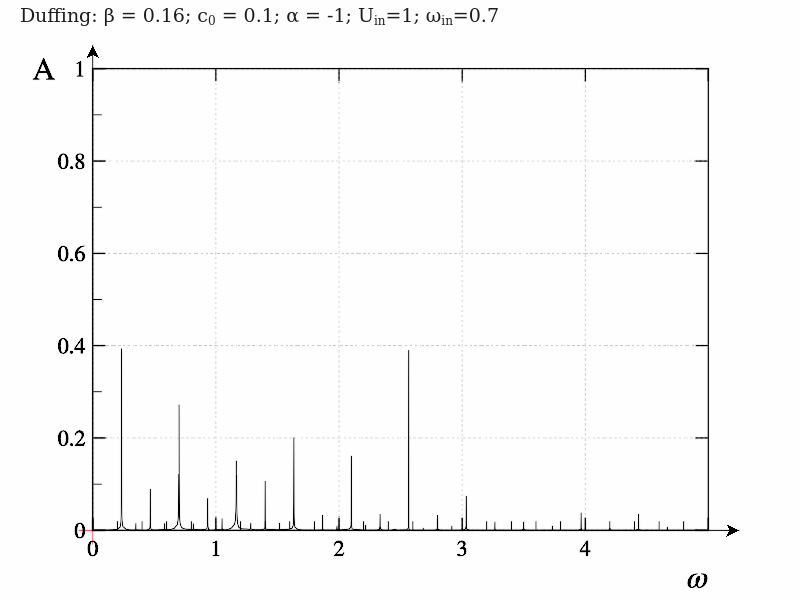
\includegraphics[width=0.49\textwidth]{p/cha/duff/duff_f_1x00_0x70_0x16.png}
\end{center}
\caption{Розширений фазовий портрет і спектр системи Дуффінга (\ref{atu:eq:duff}) в режимі складно-періодичних коливань}
\label{atu:f:duff_phase_f_reg}
\end{figure}

Малі зміни параметра
$ \beta $ можуть перевести систему в режим хаотичних коливань, при
яких частота вхідного сигналу відображається яскраво вираженим піком
(рис.~\ref{atu:f:duff_phase_f_chaos1}). Також виражені третя і п'ята гармоніка
вхідного сигналу, а ділянка суцільного спектра виражена слабо.

\begin{figure}[ht!]
\begin{center}
  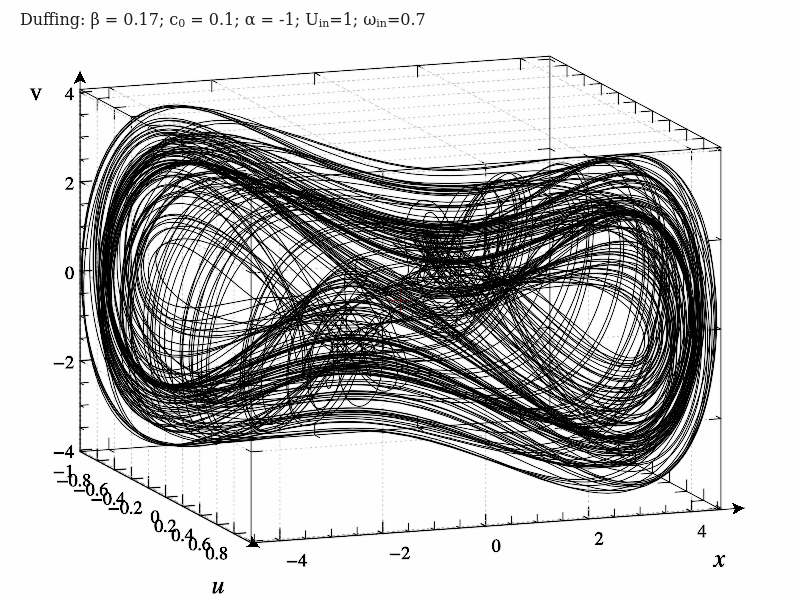
\includegraphics[width=0.49\textwidth]{p/cha/duff/duff_p_1x00_0x70_0x17.png}
  \hfill
  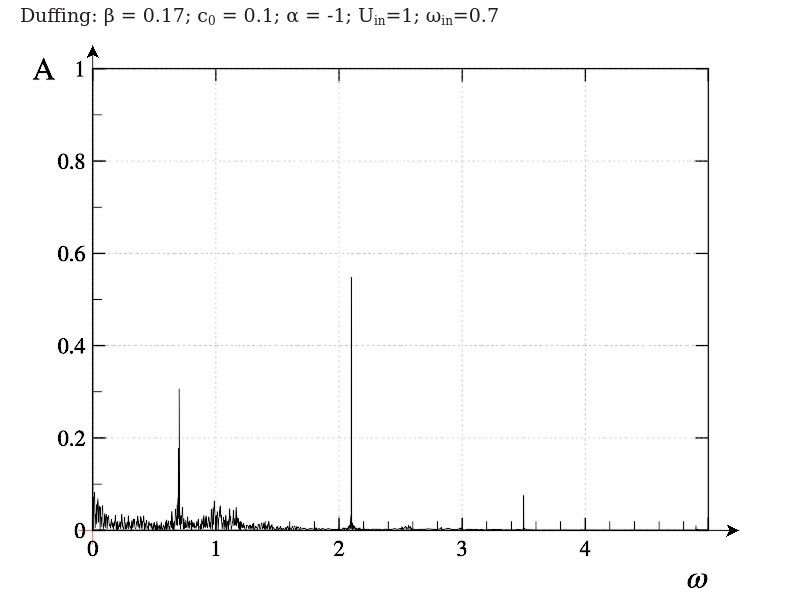
\includegraphics[width=0.49\textwidth]{p/cha/duff/duff_f_1x00_0x70_0x17.png}
\end{center}
\caption{Розширений фазовий портрет і спектр системи Дуффінга (\ref{atu:eq:duff}) в режимі слабо виражених хаотичних коливань}
\label{atu:f:duff_phase_f_chaos1}
\end{figure}


При подальшому зростанні параметра
$ \beta $ відбувається чергування хаотичного і складно-періодичного
режимів. Існують ділянки, на яких стабільно спостерігається
хаотичний режим, при цьому ділянки суцільного спектра виражені значно
сильніше~(рис.~\ref{atu:f:duff_phase_f_chaos2}).

\begin{figure}[ht!]
\begin{center}
  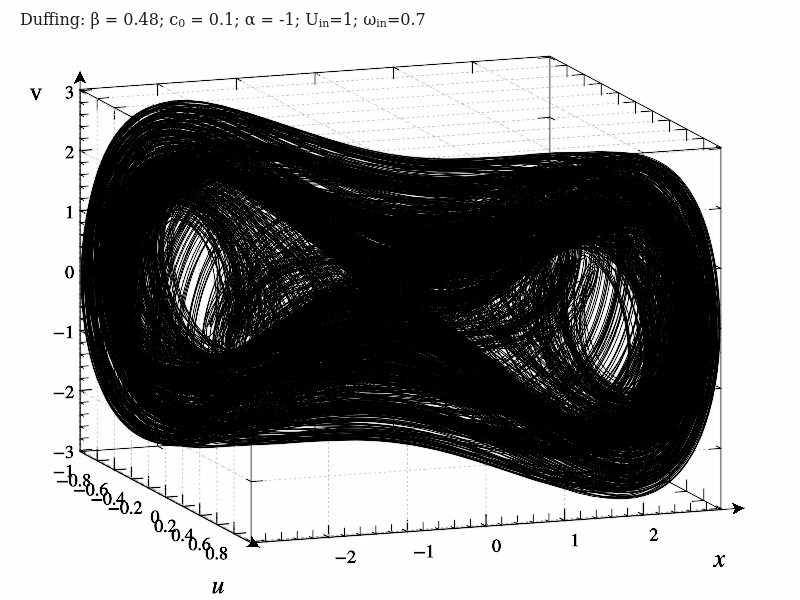
\includegraphics[width=0.49\textwidth]{p/cha/duff/duff_p_1x00_0x70_0x48.png}
  \hfill
  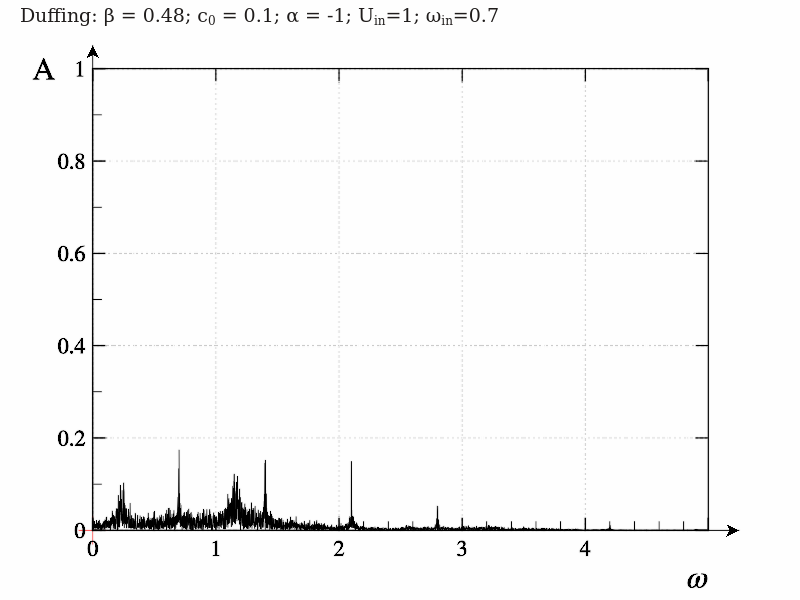
\includegraphics[width=0.49\textwidth]{p/cha/duff/duff_f_1x00_0x70_0x48.png}
\end{center}
\caption{Розширений фазовий портрет і спектр системи Дуффінга (\ref{atu:eq:duff}) в режимі виражених хаотичних коливань}
\label{atu:f:duff_phase_f_chaos2}
\end{figure}

Аналіз спектру системи в хаотичному режимі дає важливе
спостереження: ділянка суцільного спектра впритул примикає
до осі ординат. Таким чином немає такої частоти, нижче якої
не спостерігалося власна динаміка системи, а виявлялися б
тільки наслідки зміни ідентифікованого параметра.
Зазвичай це приводить до певних
складнощів при усередненні критеріїв ідентифікації.

% }}}2

\subsection{Аналіз і вибір критерію} % {{{2

Розглянемо можливості визначення виду критерію, ґрунтуючись на
фізичних принципах. Досліджувана система через малу величину
\(c_0\) дуже близька до консервативної, і спостережувані зміни
повної енергії системи в основному обумовлені взаємодією з
зовнішнім джерелом енергії --- вхідним сигналом~$u(t)$.

Перш за все зазначимо, що при незмінних параметрах системи і
вхідного сигналу, не дивлячись на те, що система і її оточення
постійно обмінюються енергією, середнє значення повної енергії
системи залишається постійним. У повну енергію вносять свій
внесок кінетична
%
\begin{equation}
E_k = m \frac{\dot{x}^2(t)}{2}
\label{atu:eq:duff_Ek}
\end{equation}
%
і потенційна енергія
%
\begin{equation}
E_p = \int\limits_0^x ( k_1 x + k_3 x^3 ) dx =
\frac{k_1 x^2}{2} + \frac{k_3 x^4}{4}.
\label{atu:eq:duff_Ep}
\end{equation}

Як випливає з (\ref{atu:eq:duff_Ep}), величина $\beta$, що ідентифікується
(в розмірному вигляді їй відповідає параметр $k_3$), безпосередньо
входить тільки в вираз для потенційної енергії, причому її
вплив найбільший при максимальних значеннях $x(t)$.
Здавалося б, що в якості величини, що визначає критерій
ідентифікації, можна було б взяти максимальне значення
вихідного сигналу при нульовому вході, так як при цьому
кінетична енергія системи нульова, і створюються сприятливі
умови для ідентифікації. Однак, це досить рідкісні випадки, щоб
на їх основі будувати надійно працюючу систему ідентифікації,
і природно, виникає питання про точність вимірювань таких
рідкісних подій.

Скористаємося тим, що вплив параметра \(\beta \) найбільш істотно проявляється
при максимальних значеннях \(x \), і, отже, в першу чергу впливає
на величину
%
\begin{equation}
 P = \frac{1}{\tau}\int\limits_0^\tau x^2(t) dt ,
\label{atu:eq:duff_P}
\end{equation}
%
де \(\tau \) --- досить великий інтервал усереднення. У свою чергу,
цю величину просто вимірювати, через велике значення \(\tau \)
(зазвичай порядку декількох десятків періодів вхідного сигналу)
вплив шумів вимірювання мінімальний.

Таким чином, в якості критерію має сенс використовувати
$q_{x^2}$ та
$q_{|x|}$. При цьому, з огляду на близької до гіперболічної
залежності має сенс включити в розгляд і критерій
$q_{x^{-2}} $. Зазначені залежності, отримані при моделюванні
динаміки системи~(\ref{atu:eq:duff}) представлені на рис.~\ref{atu:f:duff_q}.

\begin{figure}[ht!]
\begin{center}
  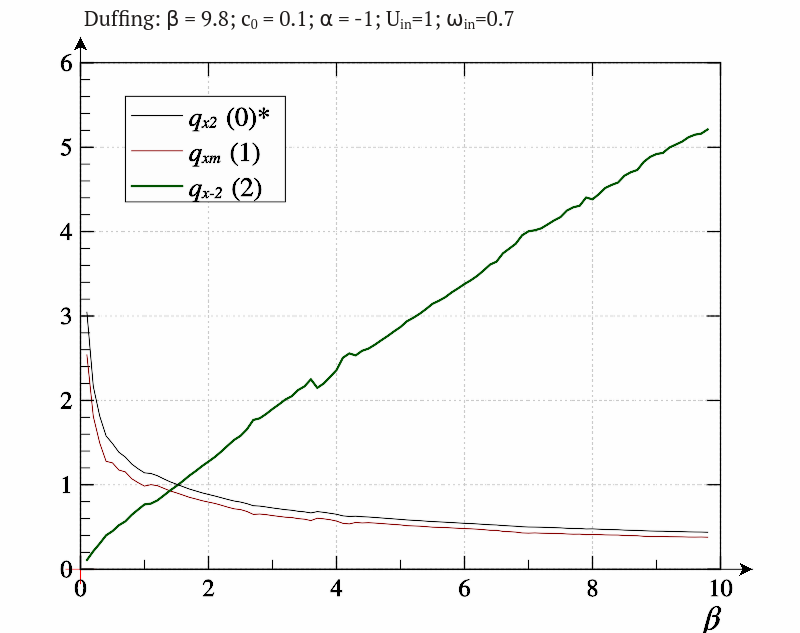
\includegraphics[width=0.49\textwidth]{p/cha/duff/duff_q-p_q_1x00_0x70.png}
\end{center}
\caption{Залежності $ q_{x^2}(\beta)$, $ q_{|x|}(\beta)$, і $q_{x^{-2}}(\beta)$ для системи Дуффінга}
\label{atu:f:duff_q}
\end{figure}

Аналіз графіків дозволяє зробити висновок, що критерій
$q_{x^{-2}}$ найбільш придатний для проведення ідентифікації. При
цьому спостерігаються невеликі порушення монотонності, що
потенційно має привести до зростання похибки ідентифікації в
околах цих порушень.



% }}}2

\subsection{Тестова задача ідентифікації для системи Дуффінга} % {{{2

При синтезу системи ідентифікації використовувалася група
методів ``ql3rlWvnAAW'' при використанні критерію
$q_{x^{-2}}$. Значення параметрів вибиралися так, що б забезпечити
наявність всіх видів коливань в робочому діапазоні:
$U_{in} = 1.0 $,
$\omega_{in} = 0.7 $,
$\beta \in [1, 4] $.

Розглянемо процес ідентифікації в квазістаціонарному випадку,
при повільної зміні параметра~(\ref{atu:eq:po_t_ramp}),
$ p_0 = 1 $,
$ U_p = 2 $. Динаміка агентів і різних способів визначення
$ p_\mathrm{id} $ представлена на рис.~\ref{atu:f:duff_id_ramp}.

\begin{figure}[ht!]
\begin{center}
  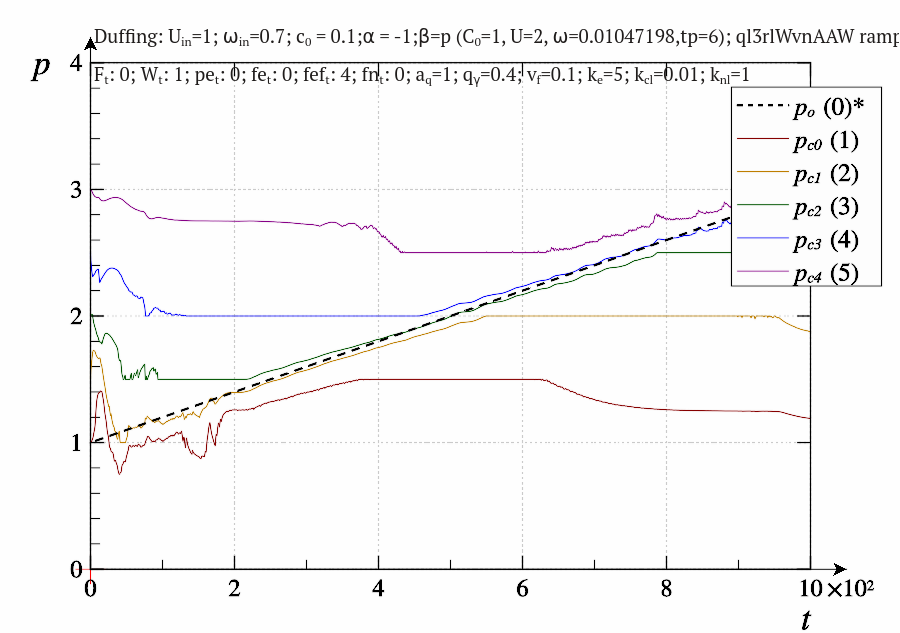
\includegraphics[width=0.49\textwidth]{p/cha/duff/duff_id-p_t_pi_ql3rlWvnAAW_ramp.png}
  \hfill
  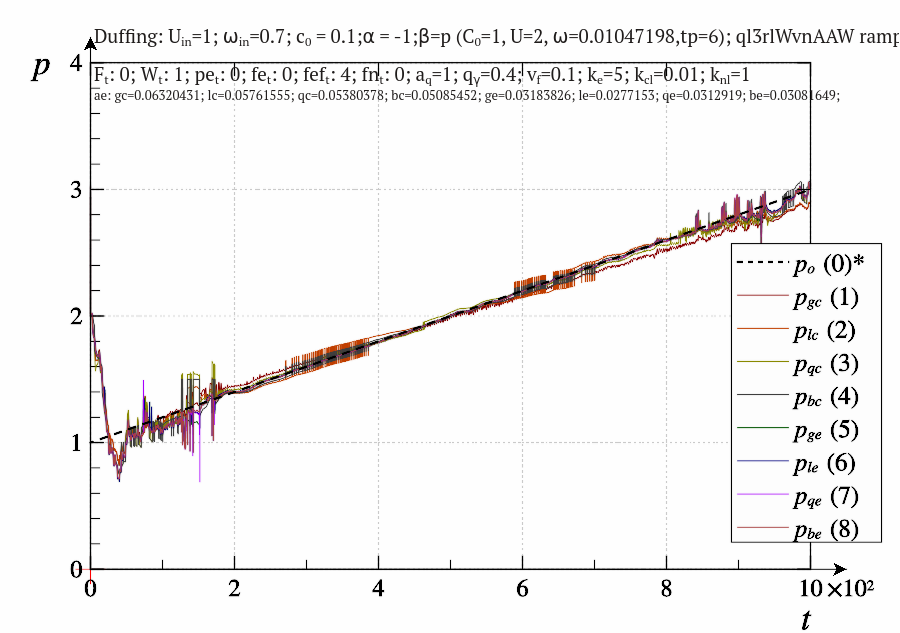
\includegraphics[width=0.49\textwidth]{p/cha/duff/duff_id-p_t_p_ql3rlWvnAAW_ramp.png}
\end{center}
\caption{Динаміка агентів і ідентифікованого значення для системи Дуффінга за умови (\ref{atu:eq:po_t_ramp})}
\label{atu:f:duff_id_ramp}
\end{figure}

Як і для попередніх систем, метод ідентифікації демонструє свою
працездатність у всьому робочому діапазоні. Але спостерігається
і суттєва відмінність. Особливості спектра системи не дають
можливості побудувати досить ефективний фільтр. Як наслідок,
у значеннях
$ p_\mathrm{id} $ спостерігаються високочастотні коливання. Найбільш
схильні до цього явища методи координаторів
$ p_{lc} $ і
$ p_{bc} $.

Розглянемо реакцію системи ідентифікації на стрибкоподібні
зміни параметра, динаміка яких була задана (\ref{atu:eq:po_t_sign}),
$p_0=2$, $U_p=0.8$, $\omega_{in}=0.01047$.
Результати представлені на рис.~\ref{atu:f:duff_id_sign}.

\begin{figure}[ht!]
\begin{center}
  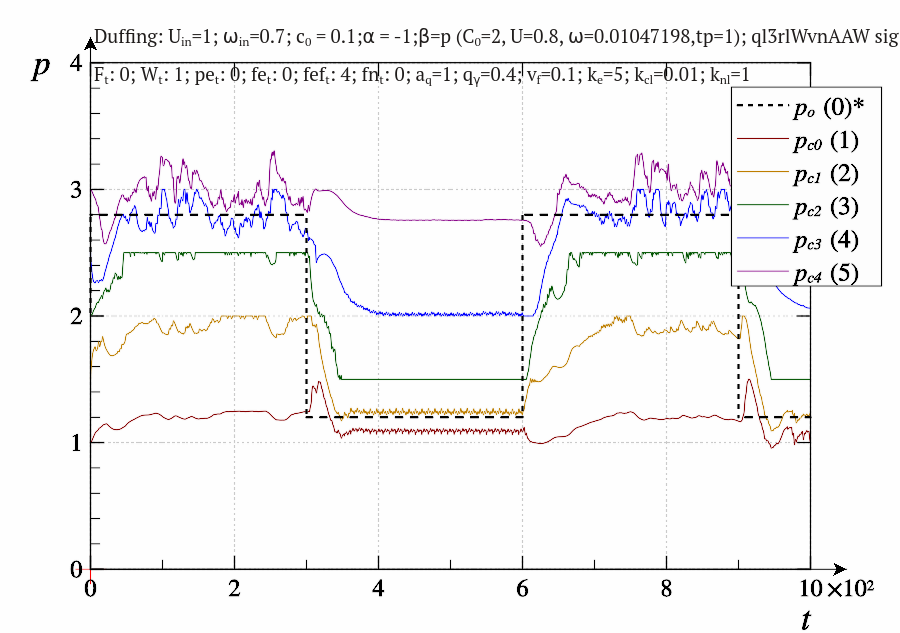
\includegraphics[width=0.49\textwidth]{p/cha/duff/duff_id-p_t_pi_ql3rlWvnAAW_sign.png}
  \hfill
  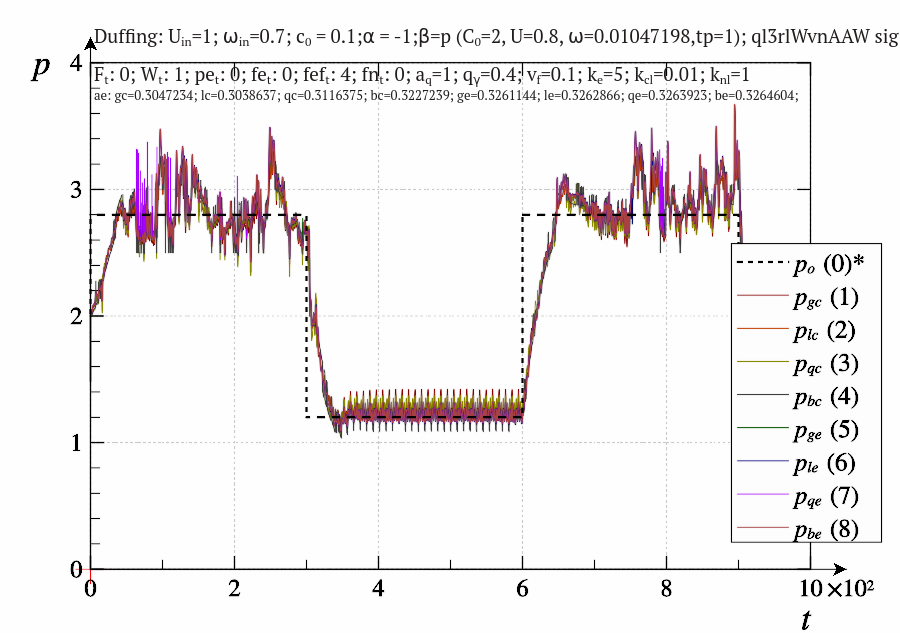
\includegraphics[width=0.49\textwidth]{p/cha/duff/duff_id-p_t_p_ql3rlWvnAAW_sign.png}
\end{center}
\caption{Динаміка агентів і ідентифікованого значення для системи Дуффінга за умови (\ref{atu:eq:po_t_sign})}
\label{atu:f:duff_id_sign}
\end{figure}

Крім вже зазначеної особливості, що полягає в підвищеному рівні
коливань, звертає на себе факт збільшення похибки ідентифікації
при
$ \beta \approx 3 $. У цій області значень параметра спостерігається
стійкий хаотичний режим, з суцільним спектром аж до нульової частоти.

При більш плавнії динаміці параметра (\ref{atu:eq:po_t_sin}),
$ p_0 = 2 $,
$ U_p = 0.8 $,
$ \omega_{in} = 0.01047 $ спостерігається аналогічна картина
(рис.~\ref{atu:f:duff_id_sign}), але розмах коливань істотно менше.

\begin{figure}[ht!]
\begin{center}
  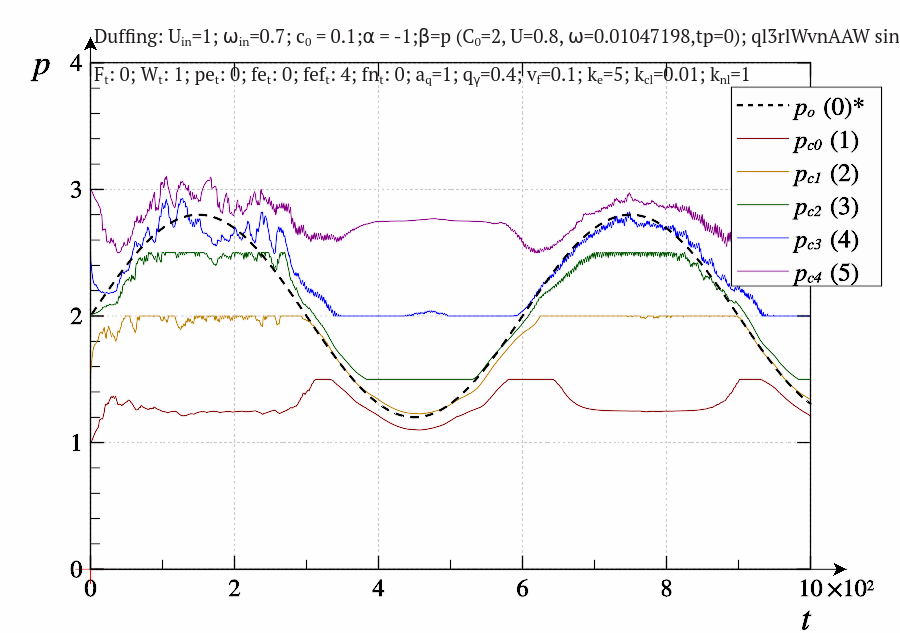
\includegraphics[width=0.49\textwidth]{p/cha/duff/duff_id-p_t_pi_ql3rlWvnAAW_sin.png}
  \hfill
  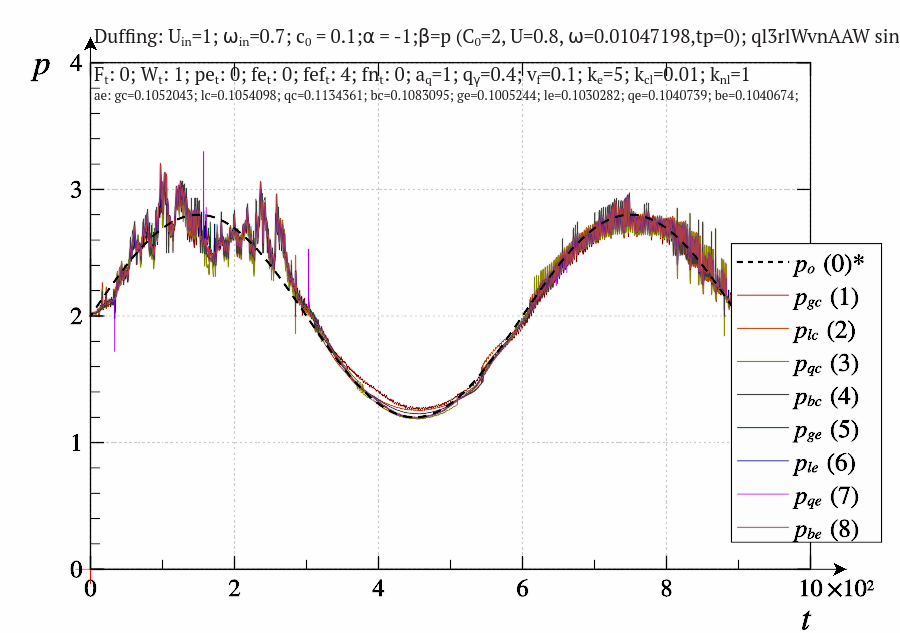
\includegraphics[width=0.49\textwidth]{p/cha/duff/duff_id-p_t_p_ql3rlWvnAAW_sin.png}
\end{center}
\caption{Динаміка агентів і ідентифікованого значення для системи Дуффінга за умови (\ref{atu:eq:po_t_sin})}
\label{atu:f:duff_id_sin}
\end{figure}


% }}}2

\subsection{Вплив параметрів системи ідентифікації на похибку ідентифікації для системи Дуффінга} % {{{2

На перший погляд, відсутність обмеження на спектр системи
знизу має відбитися на залежності помилок ідентифікації від
параметра усереднення критерію
$a_q$. Однак, ці залежності, отримані в результаті чисельного
експерименту, та представлені на рис.~\ref{atu:f:duff_e_a_q}, свідчать про
зворотне. Вид цих залежностей є цілком типовим для подібних
систем. Положення мінімуму похибки визначається динамікою
ідентифікованого параметра.

\begin{figure}[ht!]
\begin{center}
  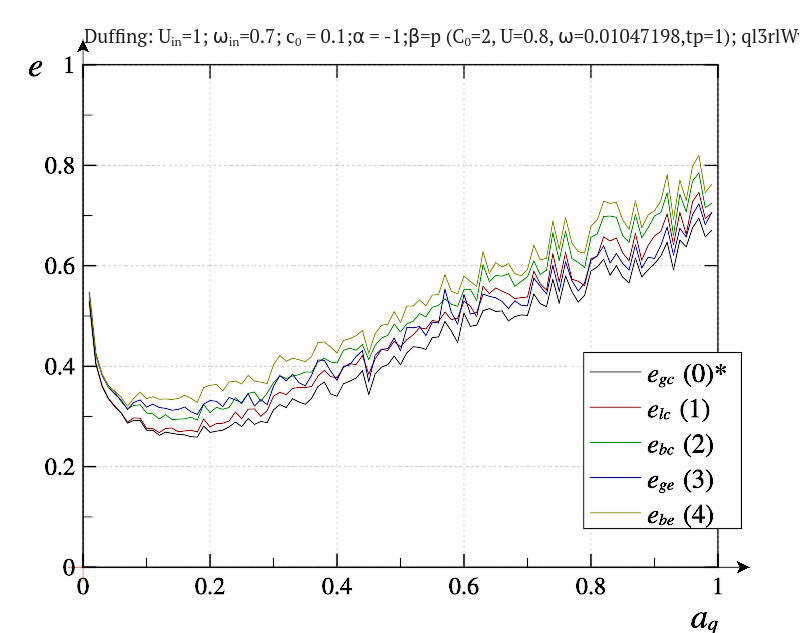
\includegraphics[width=0.49\textwidth]{p/cha/duff/duff_id-p_a_q_sign.png}
  \hfill
  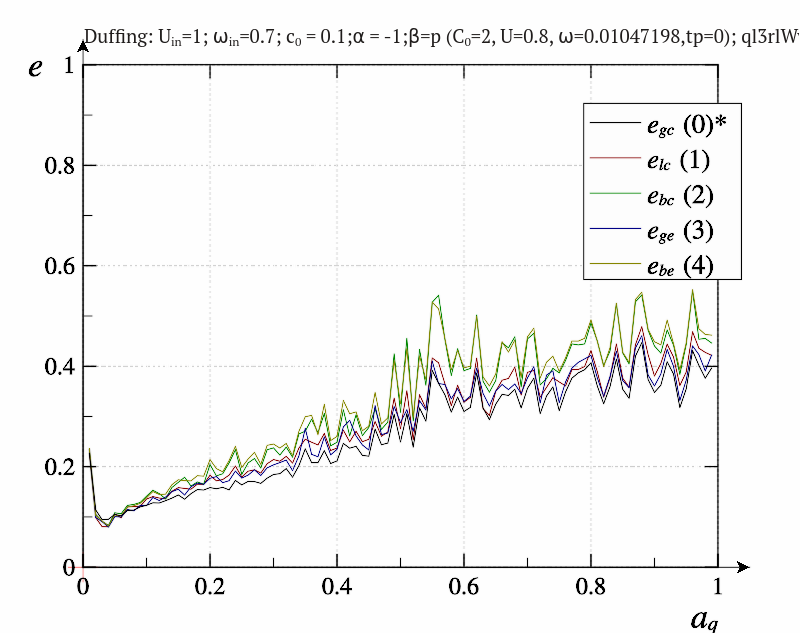
\includegraphics[width=0.49\textwidth]{p/cha/duff/duff_id-p_a_q_sin.png}
\end{center}
\caption{Залежності $ \bar{e} (a_q) $ для системи Дуффінга}
\label{atu:f:duff_e_a_q}
\end{figure}

Залежності
$ \bar{e} (q_\gamma) $ для системи Дуффінга, наведені на
рис.~\ref{atu:f:duff_e_q_gamma}, також не виділяються нічим особливим.

\begin{figure}[ht!]
\begin{center}
  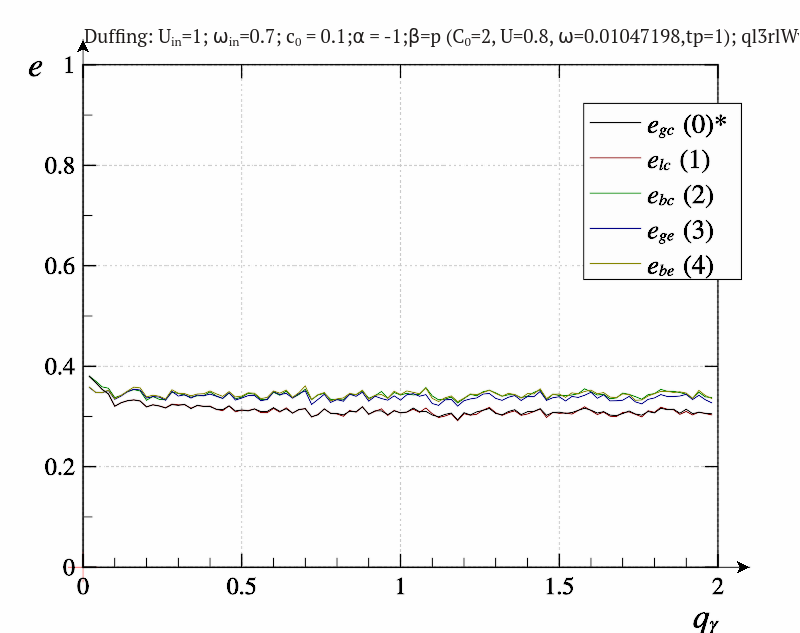
\includegraphics[width=0.49\textwidth]{p/cha/duff/duff_id-p_q_gamma_sign.png}
  \hfill
  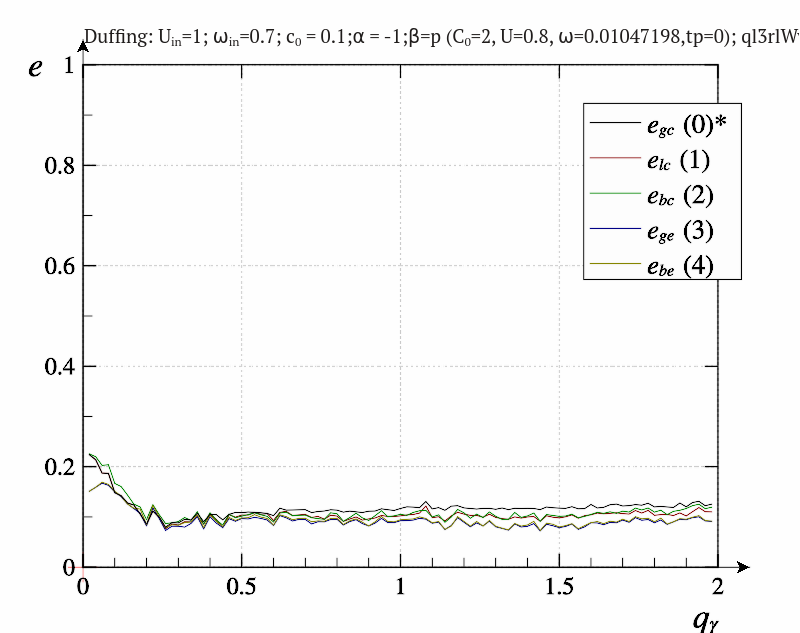
\includegraphics[width=0.49\textwidth]{p/cha/duff/duff_id-p_q_gamma_sin.png}
\end{center}
\caption{Залежності $ \bar{e} (q_\gamma) $ для системи Дуффінга}
\label{atu:f:duff_e_q_gamma}
\end{figure}

При слабше вираженої динаміці параметра ефект надмірної
чутливості більш виражений. Для сильно вираженої динаміки
спостерігається досить дивне явище --- несподівано малу похибку
ідентифікації забезпечує метод~$p_{gc}$.

Залежності похибки ідентифікації від коефіцієнта швидкості $ v_f $ представлені на рис.~\ref{atu:f:duff_e_v_f}.

\begin{figure}[ht!]
\begin{center}
  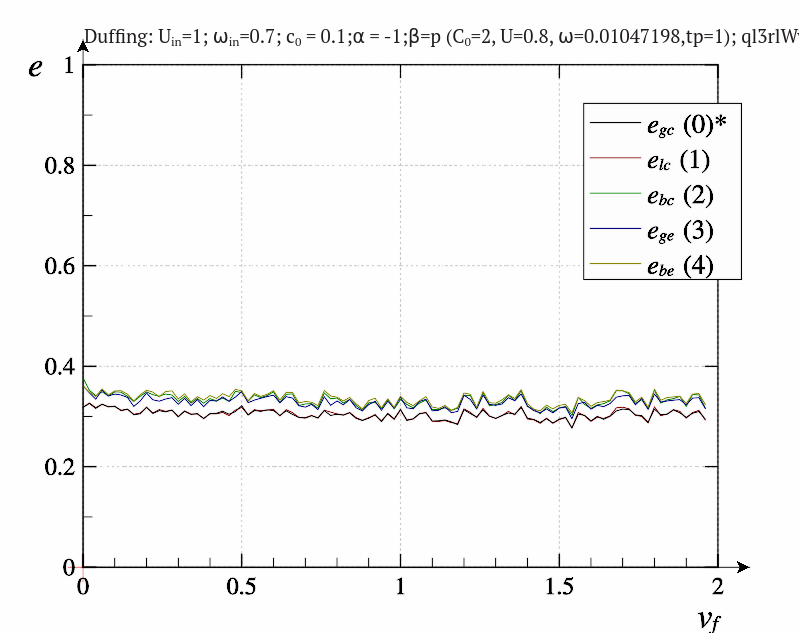
\includegraphics[width=0.49\textwidth]{p/cha/duff/duff_id-p_v_f_sign.png}
  \hfill
  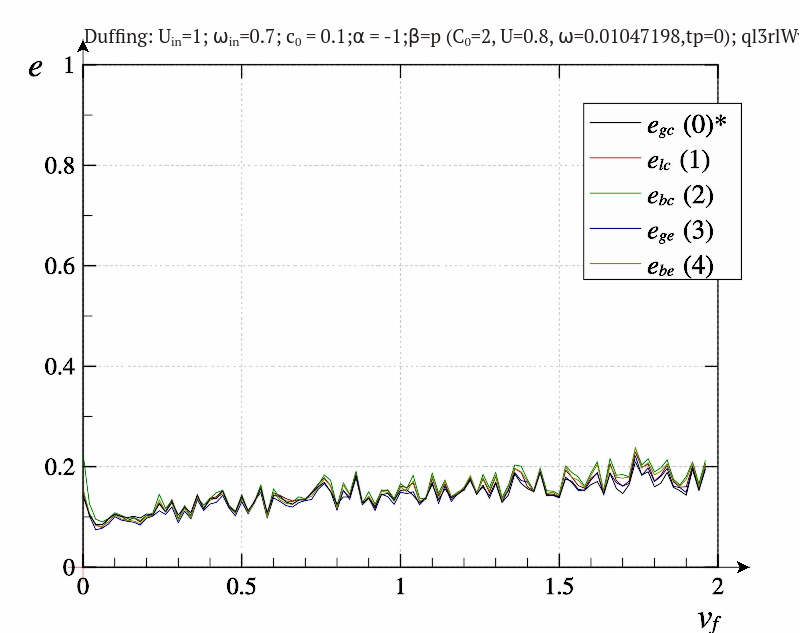
\includegraphics[width=0.49\textwidth]{p/cha/duff/duff_id-p_v_f_sin.png}
\end{center}
\caption{Залежності $ \bar{e} (v_f) $ для системи Дуффінга}
\label{atu:f:duff_e_v_f}
\end{figure}

Вид цих залежностей підкреслює меншу користь від зсуву агентів
при вираженій динаміці ідентифікованого параметра. Для
синусоїдальної залежності (\ref{atu:eq:po_t_sin}) максимальний виграш
від зсуву агентів досягає 120\%, для меандру --- не більше~10\%.

Залежності
$ \bar{e} (k_e) $ для системи Дуффінга (рис.~\ref{atu:f:duff_e_k_e}) демонструють
подібну поведінку, при цьому цей коефіцієнт має непрямий
вплив за швидкість зсуву агентів, основний вплив він робить на
рівноважне їх становище.

\begin{figure}[ht!]
\begin{center}
  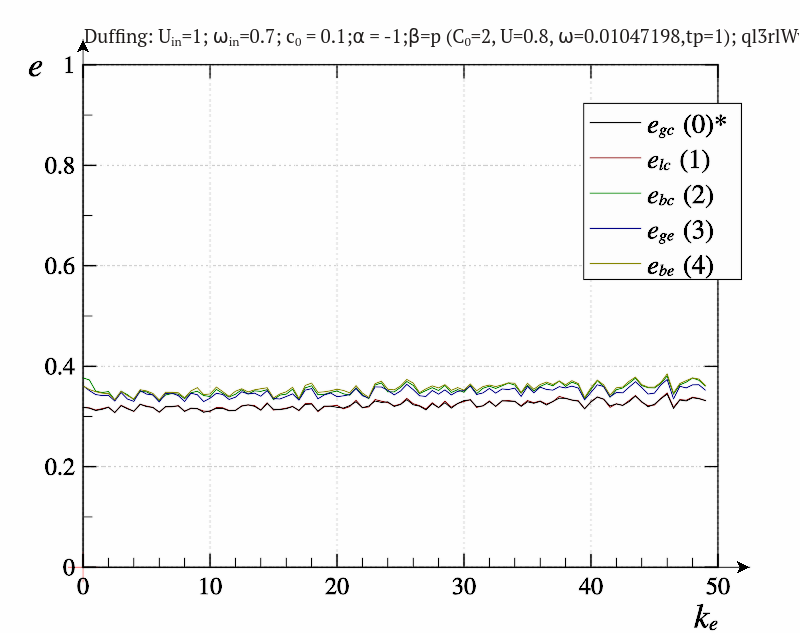
\includegraphics[width=0.49\textwidth]{p/cha/duff/duff_id-p_k_e_sign.png}
  \hfill
  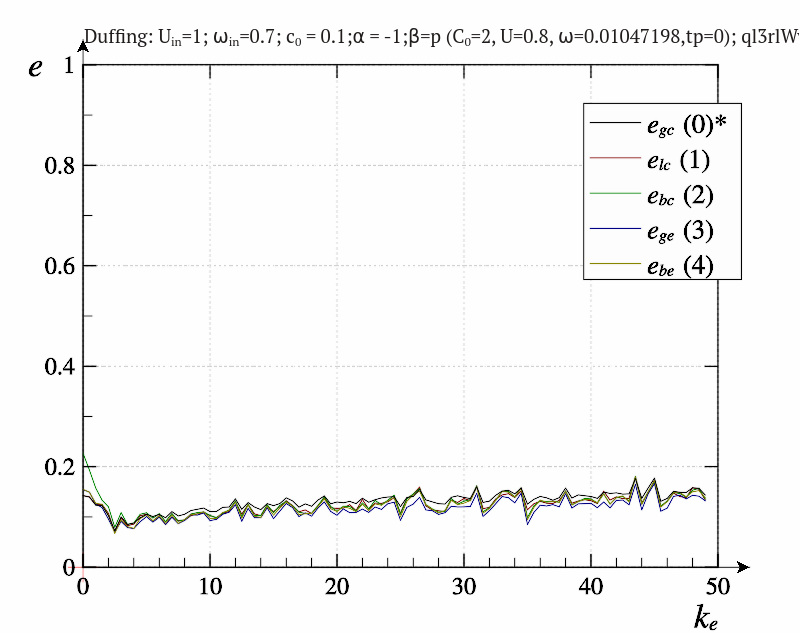
\includegraphics[width=0.49\textwidth]{p/cha/duff/duff_id-p_k_e_sin.png}
\end{center}
\caption{Залежності $ \bar{e} (k_e) $ для системи Дуффінга}
\label{atu:f:duff_e_k_e}
\end{figure}

Залежності $ \bar{e} (k_{nl}) $ для системи Дуффінга (рис.~\ref{atu:f:duff_e_k_nl}) досить
слабо виражені, з огляду на вже згадані властивості системи.


\begin{figure}[ht!]
\begin{center}
  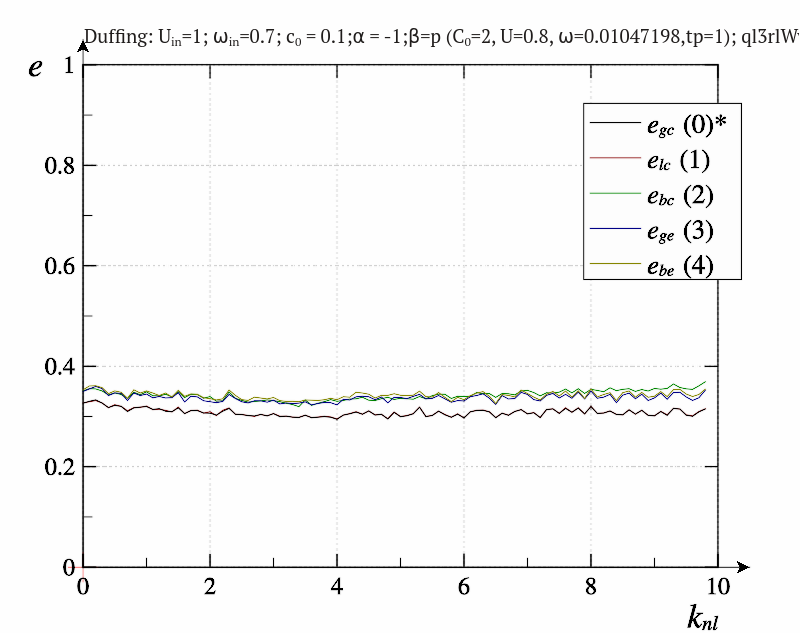
\includegraphics[width=0.49\textwidth]{p/cha/duff/duff_id-p_k_nl_sign.png}
  \hfill
  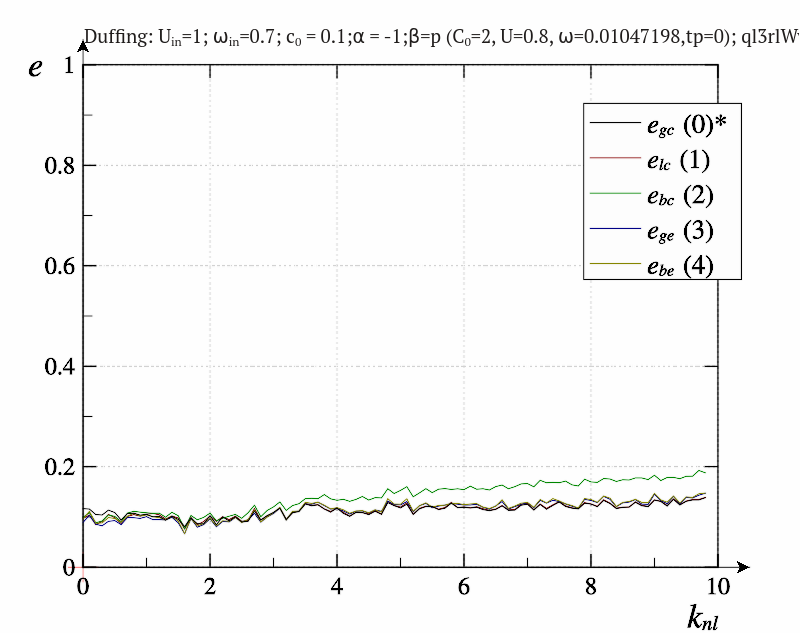
\includegraphics[width=0.49\textwidth]{p/cha/duff/duff_id-p_k_nl_sin.png}
\end{center}
\caption{Залежності $ \bar{e} (k_{nl}) $ для системи Дуффінга}
\label{atu:f:duff_e_k_nl}
\end{figure}

Вплив коефіцієнта
$ k_{cl} $ на похибку ідентифікації, в умовах штучних обмежень
на зміщення агентів, продовжує залишатися незначним
(рис.~\ref{atu:f:duff_e_k_cl}).

\begin{figure}[ht!]
\begin{center}
  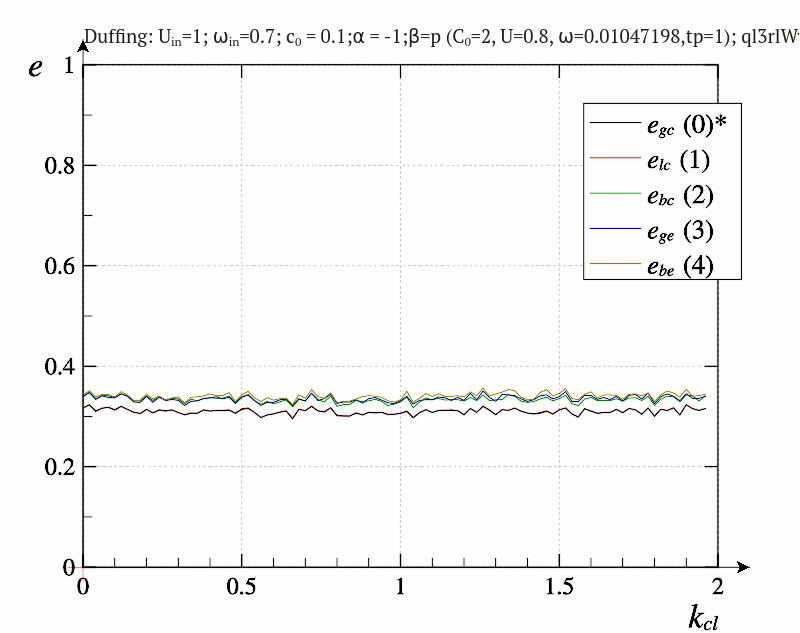
\includegraphics[width=0.49\textwidth]{p/cha/duff/duff_id-p_k_cl_sign.png}
  \hfill
  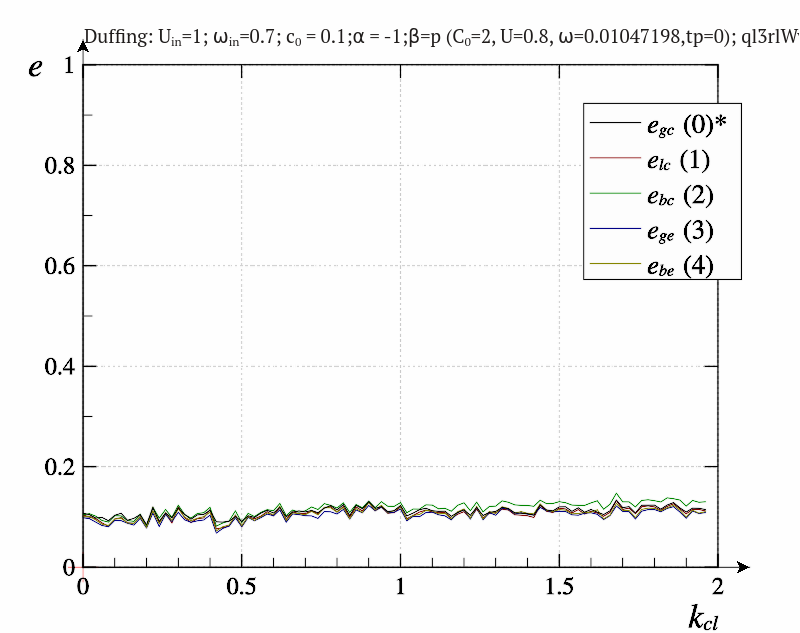
\includegraphics[width=0.49\textwidth]{p/cha/duff/duff_id-p_k_cl_sin.png}
\end{center}
\caption{Залежності $ \bar{e} (k_{cl}) $ для системи Дуффінга}
\label{atu:f:duff_e_k_cl}
\end{figure}


% }}}2

\subsection{Висновки}%{{{2

Результати моделювання процесів ідентифікації параметра
``$\beta$'' системи Дуффінга дозволяють в зробити наступні висновки:

\begin{itemize}

  \item
    Критерій
    $q_{x^{-2}}$ підходить для ідентифікації параметра ``$\beta$'' системи
    Дуффінга в широкому діапазоні, відповідні залежності проявляють
    слабку чутливість до перебудови динаміки системи.

  \item
    Наявність суцільного спектра системи, що примикає до нульової
    частоті, ускладнює визначення коректного усереднення критерію,
    що призводить до високочастотних коливань значення
    $ p_\mathrm{id} $, при їх обмеженій амплітуді.

  \item
    Група методів ql3rlWvnAAW в черговий раз показала свою добру
    працездатність.


\end{itemize}


% }}}2

% }}}1

% vim: fdm=marker foldlevel=1 foldignore="%#" fdc=4 ft=tex
